%%%%%%%%%%%%%%%%%%%%%%%%%%%%%%%%%%%
%%  Webseite / Front end
%%%%%%%%%%%%%%%%%%%%%%%%%%%%%%%%%%%
\section{Analyse der Webseite (front end)}

Die Webseite der Wetterstation Arbon besteht neben der Homepage aus zwölf Unterseiten. Für uns wichtig sind all jene, die mit den Sensordaten, der Webcam, oder der Datenbank in Verbindung stehen, hervorgehoben in Abbildung \ref{img:sitemap}. Im Folgenden werden die gefundenen Schwachstellen erklärt.

\begin{figure}[h!]
	\centering
	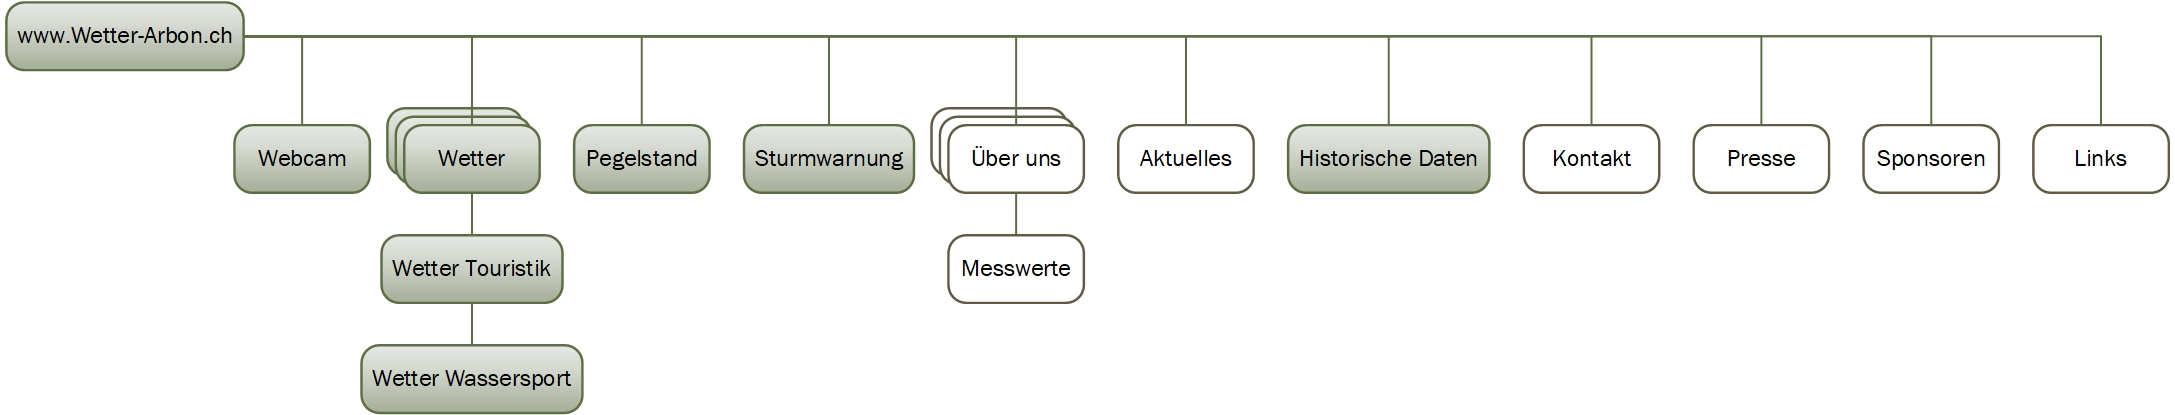
\includegraphics[width=0.9\linewidth]{img/sitemap2}
	\caption{Sitemap der Webseite}
	\label{img:sitemap}
\end{figure}


% #####################################################################################
% Browser-Kompatibilität
% ################################
\subsection{Browser-Kompatibilität}
\label{subsec:flash}
Die Anzeige der Wetterdaten erfolgt durch die Software \textit{WeatherDisplay Live}\footnote{ \url{http://www.weather-display.com/wdlive}}. WeatherDisplay Live erstellt aus den Messwerten eine Adobe Flash Applikation, welche auf der Webseite eingebettet wird, wie in Abbildung~\ref{img:responsive} dargestellt (gelb markiert).
\newline

\noindent
%\subsection*{Problem}
Adobe Flash war eine einfache Möglichkeit, animierte Grafiken auf Webseiten darzustellen und wurde praktisch von allen Browsern, nach Installation des Plug-ins, unterstützt. Diverse Sicherheitslücken und der Umstand, dass es sich um eine proprietäre, das heisst closed-source Software handelte, führten dazu, dass Apple 2010 entschied, Adobe Flash auf ihrem Mobile-Bertiebssystem \textit{iOS} nicht mehr zu unterstützen\cite{Apple:ThoughtsOnFlash}. Sämtliche Adobe Flash Animationen können somit nicht auf iPhone und iPad angezeigt werden.

Da ein Grossteil der Schweizer Bevölkerung jedoch genau diese Mobilgeräte verwendet, wurde für die Wetterstation folgender Workaround geschaffen: Der Browser prüft zuerst, ob das Gerät Adobe Flash unterstützt. Wenn ja, wird die normale Applikation geladen, wenn nicht, wird ein Printscreen der Applikation geladen. Der Nachteil dieses Workarounds ist jedoch, dass der Printscreen weder dynamisch noch interaktiv ist. Um die aktuellen Werte zu erhalten, muss die Seite jeweils neu geladen werden. Die interaktiven Elemente sind unbrauchbar, das heisst die Änderung von Einheiten, Anzeige von Rekordwerten und weiteren Graphen ist nicht möglich. Im Juli 2017 hat Adobe zudem angekündigt, dass Adobe Flash im Jahr 2020 eingestellt wird\cite{Adobe:FlashTheFutureofInteractiveContent}.
\newline

\noindent
%\subsection*{Lösungsansatz}
2014 wurde die neue HTML-Spezifikation, HTML5, fertiggestellt. HTML5 bietet diverse neue Funktionen, unter anderem im Bereich dynamischer Grafiken. Es ist der neue Web-Standard und wird von allen modernen Web-Browsern unterstützt, ohne dass irgendwelche Plug-ins installiert werden müssen. Es gibt zudem diverse Javascript-Bibliotheken wie zum Beispiel Google Charts\footnote{ \url{https://developers.google.com/chart/interactive/docs/gallery}} oder D3.js\footnote{ \url{https://github.com/d3/d3/wiki/Gallery}}, mit denen sich ansehnliche und moderne Grafiken erstellen lassen. HTML5 eignet sich somit ideal als Ersatz von Adobe Flash, um die Wetterdaten grafisch darzustellen. 


% #####################################################################################
% Barrierefreier Zugang
% ################################
\subsection{Barrierefreier Zugang}
Die Wetterstation und ihre Webseite ist eine Dienstleistung der Stadt Arbon. Sie gehört der Bevölkerung und soll deshalb für möglichst alle zugänglich sein. Sowohl die \flqq Web Content Accessibility Guidelines\frqq\footnote{ \url{https://www.w3.org/TR/2008/REC-WCAG20-20081211/}} des W3C-Konsortiums, als auch die deutsche \flqq  Barrierefreie-Informationstechnik-Verordnung\frqq\footnote{ \url{https://www.gesetze-im-internet.de/bitv_2_0/BJNR184300011.html}} bieten diverse Inputs, wie die Bedienbarkeit und somit Zugänglichkeit einer Webseite verbesserte werden kann. 
\newline

\noindent
%\subsection*{Problem}
WeatherDisplay Live, welches zum Anzeigen der Wetterdaten verwendet wird, ist eine proprietäre Software, die nur sehr eingeschränkt angepasst werden kann und auf Adobe Flash basiert. Es lassen sich beispielsweise die Anordnung der Anzeigeelemente und die Einheiten konfigurieren. Viel mehr nicht.  Adobe Flash gilt als kritische Technologie in Hinblick auf Barrierefreiheit. Mit der jetzigen Konfiguration können die Anforderung an eine barrierefreie Seite nicht umgesetzt werde.
\newline

\noindent
%\subsection*{Lösungsansatz}
Wie in Abschnitt \ref{subsec:flash} erläutert, muss WeatherDisplay Live ersetzt werden. Das bietet die Möglichkeit, dass die Entwicklung der neuen Webseite nach den oben erwähnten Richtlinien erfolgen kann.


% #####################################################################################
% Responsive Design
% ################################
\subsection{Responsive Design}
Die Webseite der Wetterstation ist mit dem Content-Management-System (CMS) \textit{Openfile64Light} der Firma Screenbox\footnote{ \url{https://screenbox.net/internet}}  erstellt. Dieses unterstützt grundsätzlich responsive Design. Das CMS gibt den Rahmen der Webseite vor. Spezielle Inhalte, wie zum Beispiel die Adobe Flash Animation, werden als sogenannte Applikationen behandelt und in die Seite eingebettet, gelb markiert in Abbildung~\ref{img:responsive}, links.
\newline

\noindent
%\subsubsection*{Problem}
Unterstützt die eingebettete Applikation kein responsive Design, so wird dieser Teil einfach linear skaliert. Dies führt dazu, dass die Anzeige der Wetterstationsdaten auf einem Mobilgerät kaum mehr lesbar sind, wie in Abbildung~\ref{img:responsive}, rechts dargestellt.
\newline

\begin{figure}[h!]
	\centering
	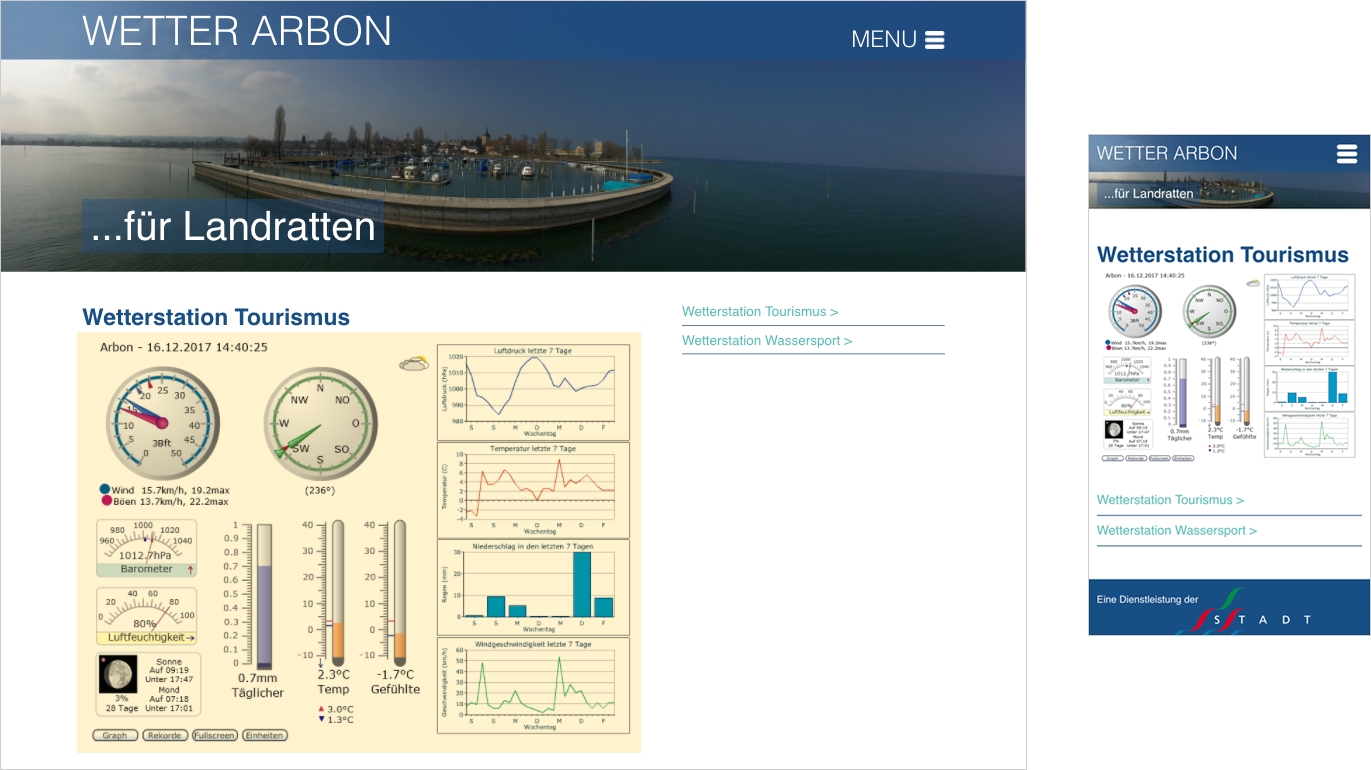
\includegraphics[width=1\linewidth]{img/responsive}
	\caption{Responsive Design: Vergleich Desktop und Mobile}
	\label{img:responsive}
\end{figure}


\noindent
%\subsubsection*{Lösungsansatz}
Mit der Adobe Flash Applikation lässt sich dieses Problem nicht lösen. Da aber, wie in Abschnitt~\ref{subsec:flash} erklärt, die Adobe Flash Applikation ohnehin abgelöst werden muss, wird bei der Ausarbeitung der neuen Anzeige darauf geachtet, dass die Wetterdaten auf allen gängigen Geräten problemlos lesbar sind. Da davon auszugehen ist, dass die Webseite häufig von Mobilgeräten aus betrachtet wird, wird das Designkonzept \textit{mobile first} angewendet. Das bedeutet, dass zuerst die Mobile-Seite designt wird und anschliessend die Desktop-Seite.


% #####################################################################################
% Darstellung der Winddaten
% ################################
\subsection{Darstellung der Winddaten}
Vielfach sind nicht nur die aktuellen Messwerte, sondern auch der Verlauf der Wetterdaten interessant. Für Segler ist beispielsweise entscheidend, wie sich die Windgeschwindigkeit über die letzten paar Stunden entwickelt hat. Auf der Webseite werden deshalb neben den aktuellen Wetterdaten ausgewählte Wetterdatenverläufe dargestellt, wie in Abbildung~\ref{img:responsive} ersichtlich. Bei diesen Grafiken geht es darum, die Tendenz und die Grössenordnung der Wetterdaten abschätzen zu können.
\newline

\begin{figure}[h!]
	\centering
	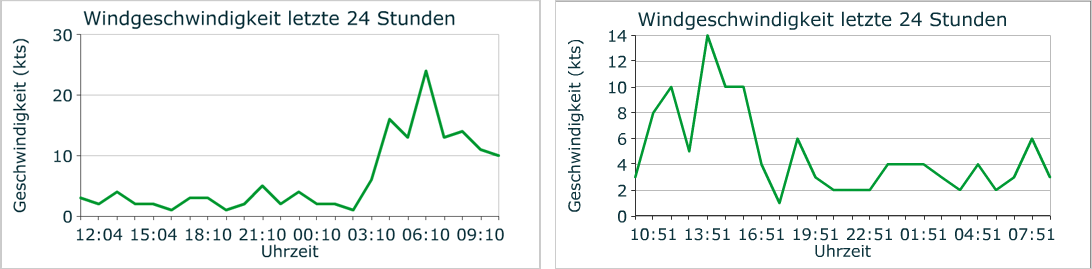
\includegraphics[width=1\linewidth]{img/wind-geschw}
	\caption{Anzeige der Windgeschwindigkeit mit variabler y-Skalierung}
	\label{img:wind-geschw}
\end{figure}

\noindent
Beim genaueren Betrachten der Verläufe von Windgeschwindigkeit und Windrichtung zeigen sich jedoch zwei Probleme.
% Windgeschwindigkeit
%\subsubsection*{Problem: Automatische y-Skalierung von Graphen}
Bei der Windstärke-Anzeige passt sich die Skalierung der y-Achse je nach Windstärke automatisch an, wie Abbildung \ref{img:wind-geschw} zeigt. Das Problem ist, dass ein schnelles Ablesen der Anzeige nicht möglich ist, da die Anzeige immer zuerst in Relation zur y-Skalierung gesetzt werden muss, was mühsam ist.
\newline



\noindent
% Windrichtung
%\subsubsection*{Problem: Sprung in der Windrichtungsanzeige}
Bei der Anzeige der Windrichtung wird der zeitliche Verlauf als Linie in einem xy-Graphen dargestellt. Die y-Achse zeigt die Himmelsrichtung an, aus der der Wind kommt von 0 Grad bis 360 Grad. Das Problem bei dieser Darstellung ist, dass, wenn der Wind über Norden dreht, dies als Sprung in der Grafik abgebildet wird, wie in Abbildung~ \ref{img:wind-richtung} dargestellt. Durch die Interpolation der Werte entsteht so eine verwirrende und falsche Aussage.
\newline

\begin{figure}[h!]
	\centering
	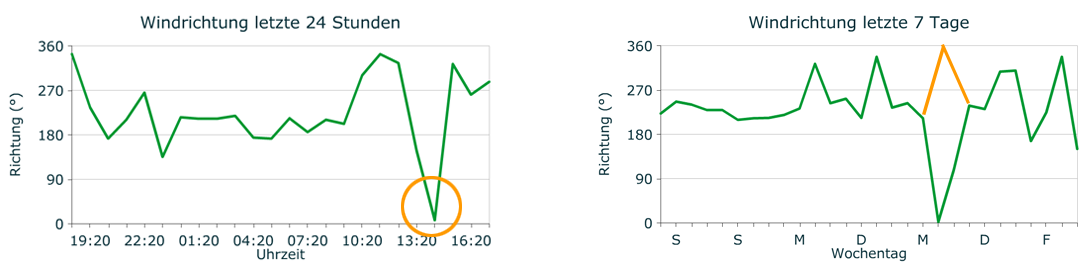
\includegraphics[width=1\linewidth]{img/wind-richtung}
	\caption{Anzeige der Windrichtung}
	\label{img:wind-richtung}
\end{figure}

\noindent
%\subsubsection*{Lösungsansatz}
Bei der Erstellung der neuen Anzeige wird darauf geachtet, dass die Graphen auf den ersten Blick eine klare Aussage zulassen, indem fixe y-Skalierungen verwendet werden. Die Auswahl der Darstellungsart erfolgt zudem so, dass keine Missverständnisse bzw. Falschaussagen entstehen.



% #####################################################################################
% Sturmwarnung
% ################################
\subsection{Integration des Sturmwarndienstes}
\label{subsec:sturmwarnung}

Auf dem Bodensee gibt es einen Sturmwarndienst, der die Schiffsführer vor aufkommendem Sturm warnen soll. Der Sturmwarndienst wird vom Deutschen Wetterdienst in Zusammenarbeit mit MeteoSchweiz betrieben. Rund um den Bodensee sind dafür über 60 Sturmwarnleuchten installiert (Abbildung \ref{img:sturm2}). Diese blinken 40 mal pro Minute bei Windböen  über 25 Knoten und 90 mal pro Minute bei Windböen über 34 Knoten. Die aktuelle Warnsituation wird zudem auf der Webseite der Kantonspolizei Thurgau\footnote{ \url{http://www.kttg.ch/kapo/htm/stwarn.shtml}} als jpg-Bild publiziert, siehe Abbildung~\ref{img:sturm}, rechts. Das jpg-Bild wird direkt auf der Webseite der Wetterstation eingebunden.
\newline

\begin{figure}[h!]
	\centering
	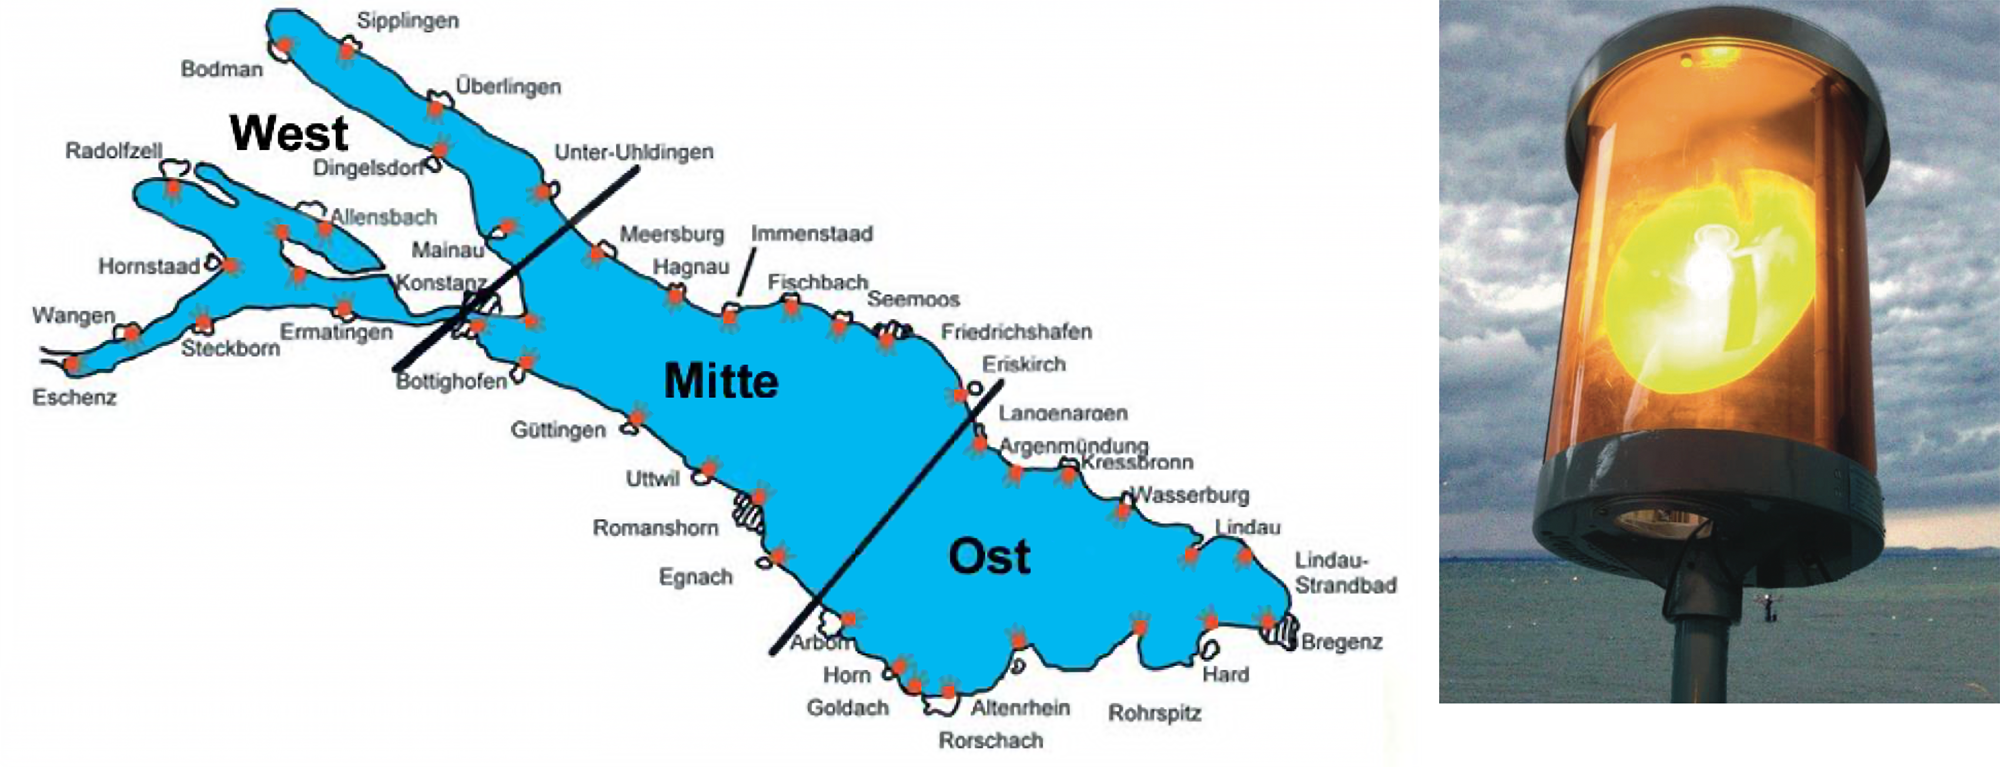
\includegraphics[width=1\linewidth]{img/sturm2}
	\caption{Sturmwarndienst Bodensee}
	\label{img:sturm2}
\end{figure}

\noindent
%\subsubsection*{Problem: HTTP}
Die Webseite der Kantonspolizei Thurgau kann nur über eine unverschlüsselte HTTP-Verbindung aufgerufen werden. Die verschlüsselte Verbindung über HTTPS wird nicht unterstützt. Google Chrome und Mozilla Firefox planen HTTP-Seiten zukünftig abzuwerten und mit einer Warnung als \flqq nicht sicher\frqq zu markieren\cite{Chromium:marking-http-as-non-secure}\cite{Mozilla:DeprecatingNon-SecureHTTP}. Für normale User ist diese Meldung nicht verständlich und erzeugt ungewolltes Misstrauen in die Webseite. 

Seit 2014 verwendet die Suchmaschine von Google zudem HTTPS als Ranking Signal. Bisher war es ein sehr schwaches Signal, das heisst die Gewichtung lag bei unter einem Prozent. Google behält sich allerdings vor, die Gewichtung zu erhöhen\cite{Googleblog:https-as-ranking-signal}. Webseiten, die nicht über HTTPS verfügen, werden somit in der Trefferliste weiter unten angezeigt.

\begin{figure}[h!]
	\centering
	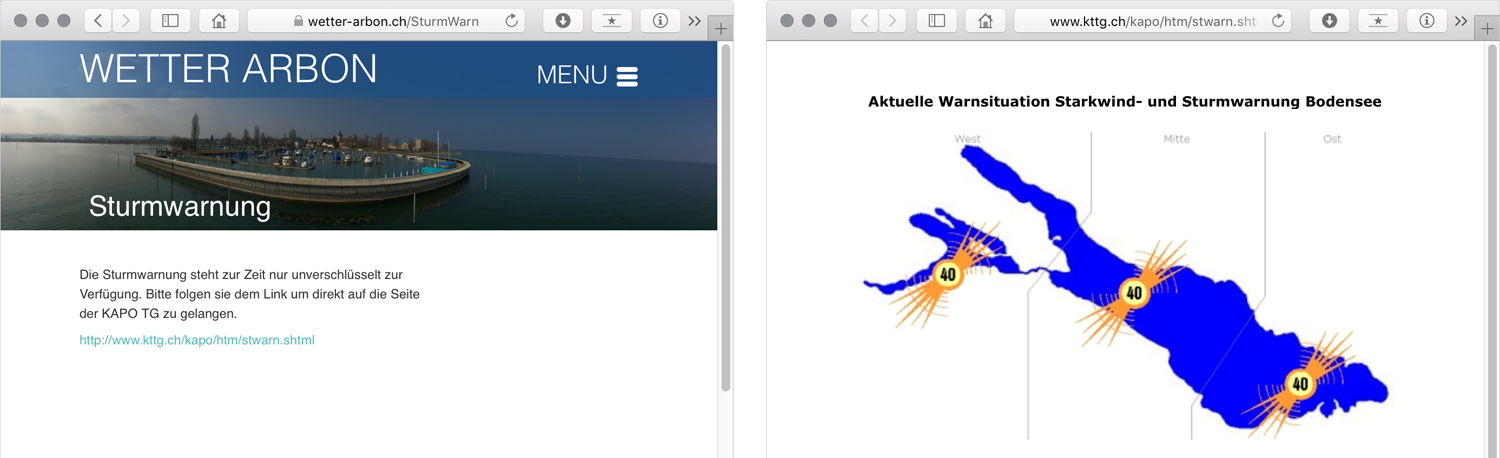
\includegraphics[width=1\linewidth]{img/sturm}
	\caption{Verlinkung der Anzeige des Sturmwarndienstes}
	\label{img:sturm}
\end{figure}

Aus diesen beiden Gründen hat Screenbox im Herbst 2017 alle Kunden aufgefordert, ihre Webseiten auf HTTPS umzustellen. Die Webseite der Wetterstation Arbon konnte problemlos umgestellt werden - mit einer Ausnahme: Da die Sturmwarnung direkt eingebettet war, konnte die Sturmwarnung-Seite der Wetterstation Arbon nicht auf HTTPS umgestellt werden. Als Sofortmassnahme wurde deshalb das eingebettete Bild entfernt und durch einen Link auf die Webseite der Kantonspolizei ersetzt, siehe Abbildung~\ref{img:sturm} links. Dass dies keine langfristige Lösung sein kann, versteht sich von selbst.

%\subsubsection*{Problem: Warnzeiten}
Der Sturmwarndienst wie in Abschnitt \ref{subsec:sturmwarnung} beschrieben, ist kein 24h-Service. Der Dienst ist nur tagsüber aktiv zu den folgenden Warnzeiten\footnote{ \url{https://kapo.tg.ch/public/upload/assets/56408/A5\%20Sturmwarnung.pdf}}, was aus Sicht der Sicherheit auf dem See nicht sehr sinnvoll ist:

\begin{itemize}  
\item 1. April - 31. Oktober: 06:00 - 22:00 Uhr 
\item 1. November - 31. März: 07:00 - 20:00 Uhr
\end{itemize}

\noindent
%\subsubsection*{Lösungsansatz}
Die Information zum Sturmwarndienst des Bodensees soll durch eine Schnittstelle abgegriffen und selbst dargestellt werden. Ob weiterhin das offizielle Signal für die Sturmleuchten, oder ein 24h-Service zum Beispiel von MeteoSchweiz verwendet werden soll, muss während der Bachelor-Arbeit mit dem Auftraggeber geklärt werden.



